\documentclass[tikz,border=6pt]{standalone}
\usepackage[T1]{fontenc}
\usepackage[utf8]{inputenc}
\usepackage{pgfplots}
\usepgfplotslibrary{groupplots}
\usetikzlibrary{calc}
\pgfplotsset{compat=1.18}
\begin{document}
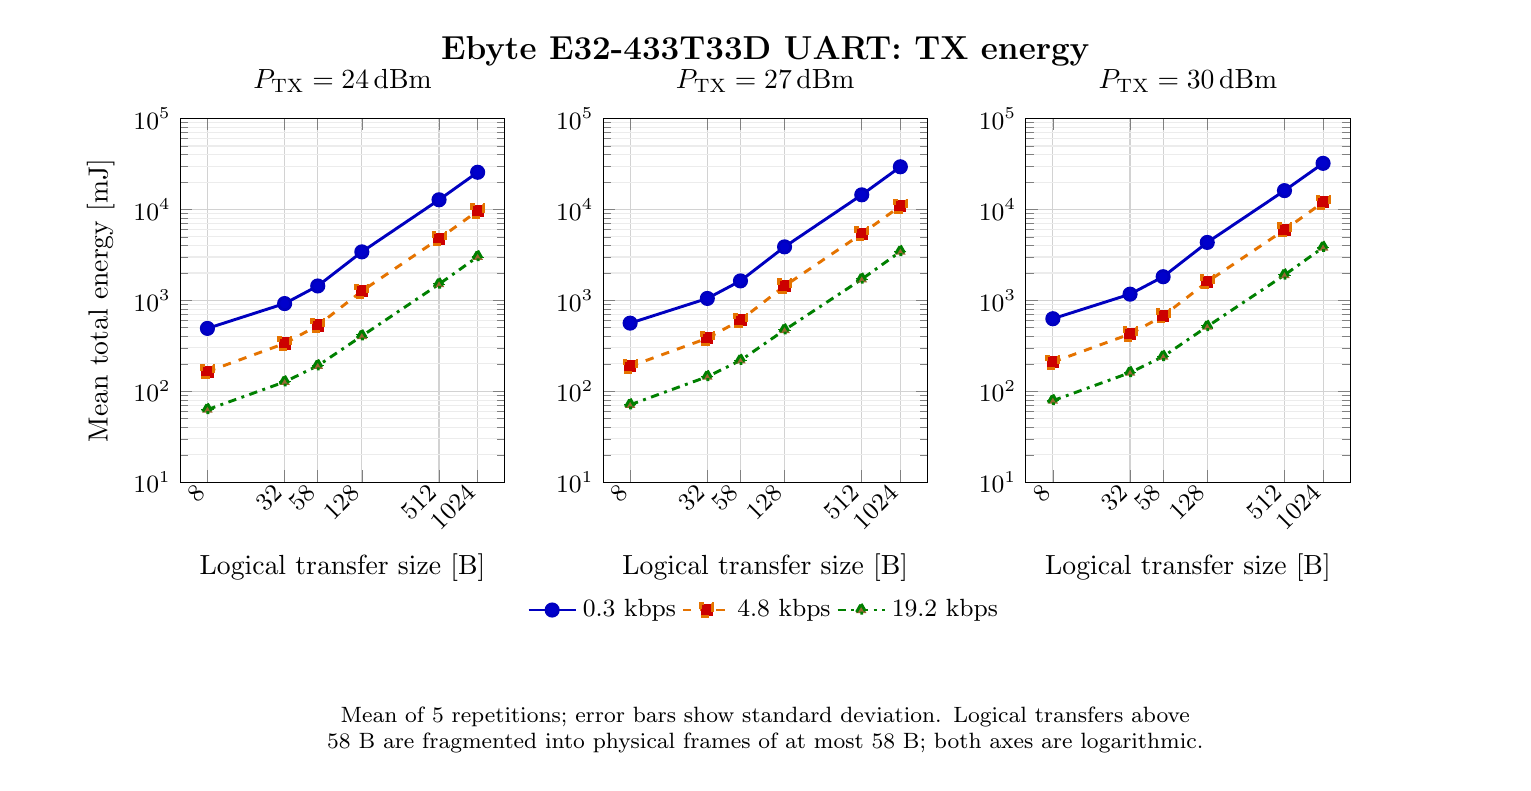
\begin{tikzpicture}
\begin{groupplot}[/pgf/number format/use comma,
  group style={group size=3 by 1, horizontal sep=1.25cm},
  width=5.7cm, height=6.2cm,
  xmode=log, log basis x={2}, ymode=log, log basis y={10},
  ymin=10, ymax=100000,
  xtick={8,32,58,128,512,1024}, xticklabels={8,32,58,128,512,1024},
  x tick label style={rotate=45, anchor=east, font=\small},
  y tick label style={font=\small},
  grid=both, minor grid style={gray!15}, major grid style={gray!35},
  xlabel={Logical transfer size [B]},
  every axis plot/.append style={line width=1.05pt},
  error bars/error bar style={line width=0.35pt},
  legend style={font=\small, draw=none, fill=none, at={(0.5,-0.29)},
    anchor=north, legend columns=-1},
]
\nextgroupplot[title={\(P_{\mathrm{TX}}=24\,\mathrm{dBm}\)}, ylabel={Mean total energy [mJ]}]
\addplot+[
  color=blue!75!black, solid, mark=*, mark size=2.2pt,
  error bars/.cd, y dir=both, y explicit,
] coordinates {
  (8,492.06372) +- (0,0.112200823)
  (32,922.817462) +- (0,0.398448772)
  (58,1441.10365) +- (0,0.696412418)
  (128,3418.71628) +- (0,1.08434348)
  (512,12786.5905) +- (0,15.3425268)
  (1024,25674.8381) +- (0,3.8584274)
};
\addplot+[
  color=orange!90!black, dashed, mark=square*, mark size=2.2pt,
  error bars/.cd, y dir=both, y explicit,
] coordinates {
  (8,164.569706) +- (0,0.0809882139)
  (32,335.958522) +- (0,0.0392959314)
  (58,529.389163) +- (0,0.276899684)
  (128,1264.94874) +- (0,0.70078365)
  (512,4775.91546) +- (0,7.71829624)
  (1024,9632.79114) +- (0,18.1600015)
};
\addplot+[
  color=green!50!black, dashdotted, mark=triangle*, mark size=2.2pt,
  error bars/.cd, y dir=both, y explicit,
] coordinates {
  (8,62.8977303) +- (0,0.0423562639)
  (32,126.882642) +- (0,0.0671759491)
  (58,190.985949) +- (0,0.1063072)
  (128,406.028354) +- (0,11.9696128)
  (512,1507.65101) +- (0,17.8296747)
  (1024,3022.51008) +- (0,46.0315153)
};
\nextgroupplot[title={\(P_{\mathrm{TX}}=27\,\mathrm{dBm}\)}]
\addplot+[
  color=blue!75!black, solid, mark=*, mark size=2.2pt,
  error bars/.cd, y dir=both, y explicit,
] coordinates {
  (8,562.099608) +- (0,0.266074816)
  (32,1050.85645) +- (0,0.296360134)
  (58,1639.20493) +- (0,0.488391346)
  (128,3881.38898) +- (0,2.3734595)
  (512,14497.0775) +- (0,36.54089)
  (1024,29489.3328) +- (0,452.033551)
};
\addlegendentry{0.3 kbps}
\addplot+[
  color=orange!90!black, dashed, mark=square*, mark size=2.2pt,
  error bars/.cd, y dir=both, y explicit,
] coordinates {
  (8,188.23853) +- (0,0.53128838)
  (32,383.569) +- (0,1.10234232)
  (58,606.214847) +- (0,0.102028802)
  (128,1440.75762) +- (0,1.11377106)
  (512,5403.04271) +- (0,9.24128146)
  (1024,10889.8528) +- (0,15.231738)
};
\addlegendentry{4.8 kbps}
\addplot+[
  color=green!50!black, dashdotted, mark=triangle*, mark size=2.2pt,
  error bars/.cd, y dir=both, y explicit,
] coordinates {
  (8,71.0552292) +- (0,0.210093121)
  (32,144.987408) +- (0,0.0755862144)
  (58,218.56276) +- (0,0.0507537785)
  (128,472.664708) +- (0,8.93545718)
  (512,1709.23597) +- (0,25.2084017)
  (1024,3442.33786) +- (0,24.8484651)
};
\addlegendentry{19.2 kbps}
\nextgroupplot[title={\(P_{\mathrm{TX}}=30\,\mathrm{dBm}\)}]
\addplot+[
  color=blue!75!black, solid, mark=*, mark size=2.2pt,
  error bars/.cd, y dir=both, y explicit,
] coordinates {
  (8,628.737694) +- (0,0.670410327)
  (32,1170.90249) +- (0,4.93153189)
  (58,1821.94434) +- (0,4.66547637)
  (128,4342.08191) +- (0,6.72239411)
  (512,16129.1662) +- (0,27.8234413)
  (1024,32183.0747) +- (0,185.95773)
};
\addplot+[
  color=orange!90!black, dashed, mark=square*, mark size=2.2pt,
  error bars/.cd, y dir=both, y explicit,
] coordinates {
  (8,209.670438) +- (0,0.266902432)
  (32,426.624127) +- (0,0.31013768)
  (58,675.06228) +- (0,1.21489628)
  (128,1599.47136) +- (0,3.51202573)
  (512,5961.70172) +- (0,18.7380437)
  (1024,11984.9281) +- (0,58.4610298)
};
\addplot+[
  color=green!50!black, dashdotted, mark=triangle*, mark size=2.2pt,
  error bars/.cd, y dir=both, y explicit,
] coordinates {
  (8,78.9158574) +- (0,0.0704566494)
  (32,160.354122) +- (0,0.138938939)
  (58,241.271356) +- (0,0.978260746)
  (128,515.970135) +- (0,18.4256201)
  (512,1902.11605) +- (0,24.9884352)
  (1024,3820.30682) +- (0,31.647345)
};
\end{groupplot}
\node[font=\bfseries\large] at ($(group c2r1.north)+(0,0.85cm)$)
  {Ebyte E32-433T33D UART: TX energy};
\node[font=\footnotesize, align=center, text width=18.5cm]
  at ($(group c2r1.south)+(0,-3.15cm)$)
  {Mean of 5 repetitions; error bars show standard deviation. Logical transfers above 58 B are fragmented into physical frames of at most 58 B; both axes are logarithmic.};
\end{tikzpicture}
\end{document}
